\documentclass[twocolumn]{article}
\usepackage[linesnumbered,ruled,longend]{algorithm2e}
\usepackage{amsmath, amssymb, amsthm}
\usepackage{multicol, relsize, geometry}
\usepackage{booktabs}
\usepackage{hyperref}
\usepackage{graphicx}
\usepackage{pgfplots}
\usepackage{pgfplotstable}
\usepackage{caption}
\usepackage{pgfplotstable}
\usepackage{indentfirst}
\usepackage{setspace}
\usepackage[none]{hyphenat}

\singlespacing
% Adjust spacing between paragraphs
\setlength{\parskip}{1ex plus 0.5ex minus 0.2ex}
\setlength\parindent{24pt}

% Add packages for font and encoding
\usepackage[T1]{fontenc}
\usepackage[utf8]{inputenc}
\usepackage{mathptmx} % Times New Roman font

% Set font size and line spacing
\usepackage{setspace}
\fontsize{10}{12}\selectfont % 10pt font size with 12pt leading
\singlespacing % Ensure single spacing within paragraphs
% Needs to be last
\usepackage[table]{xcolor}

\DontPrintSemicolon
\SetKwFor{For}{for}{do}{end for}
\SetKwIF{If}{ElseIf}{Else}{if}{then}{else if}{else}{end if}%
% Redefine \ForEach to display a vertical line under it
\SetKwFor{ForEach}{for each}{}{end for}
\geometry{top=1cm, bottom=2cm, left=1cm, right=1cm}
\newcommand{\pluseq}{\mathrel{+}=}
\title{A heterogeneous vehicle routing problem with drones and multiple depots}
\author{Panagiotis Zachos}
\date{June 2024}

\begin{document}
	\maketitle
	
	\section*{ABSTRACT}
	The rapid growth of e-commerce and the increasing demand for efficient delivery systems have underscored the importance of optimizing logistics and routing strategies. In this context, the integration of drones into last-mile delivery services is anticipated to expand significantly, fueled by technological innovations, economic advantages, and the escalating need for rapid and efficient delivery solutions. This growing relevance of drones in logistics motivates the study of novel problems that incorporate the unique capabilities and constraints of drones, aiming to enhance delivery efficiency and meet evolving customer expectations. Motivated by the above, this paper introduces a novel and complex problem within the logistics and routing sector, which we term the "Multi-Depot Mixed Fleet Capacitated TSP" (MD-mfcmTSP), whereby a set of heterogeneous vehicles located in different depots must deliver a set of homogeneous parcels to customers in the minimum time. All vehicle types have capacity measured as the parcels they can carry. A distinctive feature of this problem is the incorporation of accessibility restrictions to certain vehicles, which add significant complexity and aim to reflect real-world challenges faced by logistics companies, such as a heterogeneous fleet and delivery constraints.
	This paper aims to formalize the MD-mfcmTSP, provide a comprehensive analysis of its components, and propose both heuristic and metaheuristic approaches for its solution. By addressing this problem, we contribute to the Travelling Salesman Problem and Vehicle Routing Problem research and the field of logistics and routing by introducing a realistic and challenging problem that considers the practical limitations and requirements of different vehicle types used in last-mile delivery. The proposed algorithms have the potential to improve efficiency and reduce costs for logistics companies operating in increasingly complex delivery environments.
	\par
	In modern logistics, the efficient delivery of parcels from multiple depots to numerous customer locations is a critical challenge. This study introduces a novel routing problem that extends the characteristics of routing problems such as the PDSTSP and VRPD by incorporating multiple vehicle types and multiple depots. This hybrid problem is particularly relevant to contemporary urban logistics scenarios, where various vehicles, such as trucks, motorbikes, and drones, are deployed from multiple last-mile depots to ensure timely deliveries. The objective of this research is to minimize the total delivery time across all customers.
	\par
	
	\section*{Keywords}
	Travelling Salesman Problem, TSP, Vehicle Routing Problem, VRP, Multi-Depot Vehicle Routing Problem, MDVRP, Multiple Travelling Salesman Problem, mTSP, Flying Sidekick Travelling Salesman Problem, FSTSP, Fleet Size and Mix VRP, mfcmTSP, last-mile delivery, city logistics, drone delivery, Parallel Drone Scheduling TSP, PDSTSP, mixed fleet delivery
	
	\section{Introduction}
	TSP is undoubtedly one of the most studied problem in combinatorics with applications spanning various fields. A generic statement of TSP in graph algorithmic terms is as follows: given a weighted unidirectional fully connected graph G(V , E) and a starting vertex, define a path of minimum length such that all vertices are visited exactly once and the path ends at the starting vertex.
	
	The Traveling Salesman Problem (TSP) is a well-studied optimization problem in combinatorial optimization, where the objective is to determine the shortest possible route that visits a set of cities and returns to the origin city. With the advent of drone technology, numerous variations of the TSP have been proposed to leverage the capabilities of drones in conjunction with traditional delivery vehicles. These variations aim to optimize delivery routes, minimize operational costs, and improve overall efficiency in logistics.
	\section{Literature Review}
	The FSTSP is a generalization of the traveling salesman problem (TSP) and the vehicle routing problem (VRP).
	\subsection{Drone-related TSP}
	\subsubsection{Flying Sidekick TSP}
	The Flying Sidekick Travelling Salesman Problem (FSTSP) was first introduced by Murray \& Chu (2015), who proposed using a combination of trucks and drones to optimize parcel delivery. The FSTSP involves a truck that can deploy and retrieve a drone to perform deliveries, thus reducing the overall delivery time and improving efficiency. The authors used MILP to model the problem and employed heuristic algorithms to solve larger instances of the FSTSP. Freitas \& Penna (2018) employed a Variable Neighborhood Search (VNS) heuristic for the FSTSP, achieving substantial improvements in delivery times. Dell’Amico et al. (2019) provided new formulations for the FSTSP and demonstrated their effectiveness through extensive computational experiments, solving benchmark instances to optimality and improving upon existing solutions. Boccia et al. (2021) proposed  new integer linear programming formulations for both the FSTSP and PDSTSP and a column-and-row generation approach to handle synchronization issues between the truck and drone solving to optimizality and improving upon instances with up to 20 customers. Kuroswiski et al. (2023) presented a hybrid Genetic Algorithm combined with Mixed Integer Linear Programming (MILP) to efficiently solve the FSTSP for up to ten customers. Pilcher (2023) proposed a self-adaptive genetic algorithm and introduced a novel two-stage mutation process designed to address the complexities of the FSTSP.
	\par
	\subsubsection{Parallel Drone Scheduling TSP}
	The Parallel Drone Scheduling Traveling Salesman Problem (PDSTSP) has garnered significant attention in recent years due to its potential to revolutionize logistics and delivery systems by incorporating drones alongside traditional delivery vehicles. The PDSTSP, also introduced by Murray \& Chu in the same paper, extends the concept of the FSTSP by involving multiple drones and optimizing the delivery process through parallel drone operations. In contrast to the FSTSP, the drones act independently from the truck and launch from and return to the depot. The authors proposed a  MILP formulation and employed heuristic algorithms to solve larger instances of the PDSTSP. Mbiadou Saleu et al. (2018) proposed an iterative two-step heuristic along with a MILP formulation. Nguyen et al. (2022) proposed an efficient branch-and-cut algorithm to solve the problem. The authors broke new ground by achieving optimal solutions for instances up to 783 customers for the first time.
	\par 
	Nguyen et al. (2023) introduced a new variant of the parallel drone scheduling traveling salesman problem that aims to increase the utilization of drones, particularly for heavy item deliveries, which they termed the PDSTSP with collective drones (PDSTSP-c).
	The authors developed a two-index MILP formulation to solve small-size instances to optimality and proposed a ruin-and-recreate metaheuristic to efficiently handle larger problem instances. Montemanni et al. (2024) expanded on the research for the PDSTSP-c and introduced a MILP and constraint programming approach.
	\par 
	Constraint programming models have been effectively utilized to handle the scheduling complexities of drone-assisted TSP variants. Ham (2018) extended the PDSTSP by considering drone drops and pickups and time-window constraints for which the author proposed a constraint programming approach to handle the problem's complexity. Montemanni and Dell’Amico (2023) presented a constraint programming model for the PDSTSP, achieving optimal solutions for various instances.
	\par 
	Hybrid optimization techniques have also been explored to solve drone-assisted TSP variants. Dinh et al. (2021) proposed a hybrid ant colony optimization metaheuristic for the PDSTSP, achieving several new best-known solutions. 
	\subsubsection{TSP-D}
	Agatz et al. (2018) introduced the Travelling Salesman Problem with Drones (TSP-D). While the TSP-D shares mostly the same characteristics as the FSTSP, the key distinction between the TSP-D and the FSTSP is that the latter requires the distinctive location between launch point and recovery point of the drone, while the former allows the drone to be launched and recovered by the truck in the same location. The authors model the problem and propose an IP model which solves instances with up to 12 customers to optimality, along with several fast heuristics to solve larger instances of the problem. Yurek et al. (2018) contributed to the TSP-D research by proposing a decomposition-based iterative optimization algorithm and verified its efficiency. Ha et al. (2018) introduced and solved the min-cost TSP-D, whose objective is to minimize the total operational costs, which include  transportation costs and waiting penalties. The authors proposed a MILP formulation and two heuristic methods to solve the problem.
	\subsubsection{Other}
	Schermer et al. (2019) introduced the Traveling Salesman Drone Station Location Problem (TSDSLP), combining TSP, facility location, and parallel machine scheduling problems to minimize operational costs. 
	Kim \& Moon (2019) introduced a mixed integer programming model for the TSP with a drone station (TSP-DS), which extends the operational range of drones. 
	\par 
	% Please add the following required packages to your document preamble:
% \usepackage{booktabs}
% \usepackage{graphicx}
\begin{table*}[]
	\caption{Drone-related TSP literature}
	\resizebox{\textwidth}{!}{%
		\begin{tabular}{@{}lllcccl@{}}
		\toprule
		\textbf{Reference} & \textbf{Problem} & \textbf{Scale} & \textbf{Synchro.} & \textbf{Flight endurance} & \textbf{Capacitated} & \textbf{Solution Method} \\ \midrule
		Murray \& Chu (2015) & FSTSP & 1-Truck 1-Drone 1-Depot & Yes & Yes & No & MILP, Heuristics \\
		\midrule
		& PDSTSP & 1-Truck n-Drone 1-Depot & No & Yes & No & MILP, Heuristics \\
		\midrule
		Ha et al. (2015) & FSTSP & 1-Truck 1-Drone 1-Depot & Yes & Yes & No & MIP, Heuristics \\
		\midrule
		Freitas \& Penna (2018) & FSTSP & 1-Truck 1-Drone 1-Depot & Yes & Yes & No & IP, Heuristics \\
		\midrule
		Boccia et al. (2021) & FSTSP/PDSTSP & 1-Truck 1-Drone 1-Depot & Yes & Yes & No & MILP, Heuristics \\
		\midrule
		Dell'Amico et al. (2021) & FSTSP & 1-Truck 1-Drone 1-Depot & Yes & Yes & No & MILP \\
		\midrule
		Dell'Amico et al. (2021) & FSTSP & 1-Truck 1-Drone 1-Depot & Yes & Yes & No & Branch and bound, Heuristic  \\
		\midrule
		Kuroswiski et al. (2023) & FSTSP & 1-Truck 1-Drone 1-Depot & Yes & Yes & No & MILP, Metaheuristics \\
		\midrule
		Pilcher (2023) & FSTSP & 1-Truck 1-Drone 1-Depot & Yes & Yes & No & Self-adaptive GA \\
		\midrule
		Mbiadou Saleu et al. (2018) & PDSTSP & 1-Truck n-Drone 1-Depot & No & Yes & No & MILP, Heuristics \\
		\midrule
		Dinh et al. (2021) & PDSTSP & 1-Truck n-Drone 1-Depot & No & Yes & No & Metaheuristics \\
		\midrule
		Nguyen et al. (2022) & PDSTSP & 1-Truck n-Drone 1-Depot & No & Yes & No & MILP \\
		\midrule
		Mbiadou Saleu et al. (2022) & PDSMTSP & m-Truck n-Drone 1-Depot & No & Yes & No & MILP, Metaheuristics \\
		\midrule
		Montemanni et al. (2023) & PDSTSP & 1-Truck n-Drone 1-Depot & Yes & Yes & No & Constraint Programming  \\
		\midrule
		Nguyen et al. (2023) & PDSTSP-c & 1-Truck n-Drone 1-Depot & No & Yes & No & MILP, Metaheuristics  \\
		\midrule
		Montemanni et al. (2024) & PDSTSP-c & 1-Truck n-Drone 1-Depot & No & Yes & No & MILP, Constraint Programming \\
		\midrule
		Ham (2018) & PDSTSP$^{+DP}$ & m-Truck n-Drone 2-Depot & No & Yes & No & Constraint Programming \\
		\midrule
		Agatz et al. (2018) & TSP-D & 1-Truck 1-Drone 1-Depot & Yes & Yes & No & IP, Heuristics \\
		\midrule
		Yurek et al. (2018) & TSP-D & 1-Truck 1-Drone 1-Depot & Yes & Yes & No & MIP, Heuristics \\
		\midrule
		Ha et al. (2018) & min-cost TSP-D & 1-Truck 1-Drone 1-Depot & Yes & Yes & No & MILP, GRASP, TSP-LS \\
		\midrule
		Dorling et al. (2016) & DDPs & 0-Truck n-Drone 1-Depot & No & Yes & Yes & MILP, SA \\
		\midrule
		Ulmer \& Thomas (2018) & SDDPHF & m-Truck n-Drone 1-Depot & No & No & No & Adaptive dynamic programming \\
		\midrule
		Salama \& Srinivas (2020) & JOCR & 1-Truck n-Drone 1-Depot & Yes & Yes & No & IP, MILP, Heuristics \\
		\midrule
		Lu et al. (2022) & FDTSP & 1-Truck n-Drone 1-Depot & Yes & Yes & No & Heuristics, Metaheuristics \\
		\midrule
		Lan (2024) & TSPTWD & 1-Truck 1-Drone 1-Depot & Yes & Yes & No & Metaheuristics \\
		\bottomrule
		\end{tabular}%
	}
\end{table*}
	\subsection{VRP}
	The Vehicle Routing Problem (VRP) is a cornerstone in the field of combinatorial optimization and logistics, focusing on the optimal routing of a fleet of vehicles to service a set of customers with known demands. Since its introduction by Dantzig \& Ramser (1959), numerous variants and extensions of the VRP have been developed to address practical and complex logistics challenges.
	The Capacitated VRP (CVRP), seeks to determine the optimal set of routes for a fleet of vehicles located in a single depot node to deliver goods to a set of customers, minimizing the total cost while satisfying constraints such as vehicle capacity and customer demand. The cost is typically defined as either the total distance, time, vehicle utilization or a combination of those.
	The primary distinction between the Vehicle Routing Problem (VRP) and the Traveling Salesman Problem (TSP) lies in the capacity constraint of the vehicles. When vehicles have unlimited or sufficiently large capacity as to not restrict the movement of the vehicle(s), the CVRP effectively reduces to a multiple Traveling Salesman Problem (mTSP). Therefore, in this paper, we will refer to the CVRP simply as the VRP.
	\subsubsection{Drone-related VRP}
	The rapid advancement of drone technology has spurred significant interest in its application to logistics and transportation, particularly in addressing the complexities of last-mile delivery. Vehicle Routing Problems with Drones (VRP-D) represent an innovative extension of traditional Vehicle Routing Problems (VRP), where drones are deployed alongside traditional delivery vehicles to enhance efficiency and reduce operational costs. This integration leverages the agility and speed of drones to complement the capacity and range of trucks, presenting new challenges and opportunities in route optimization. The VRP-D and its variants focus on optimizing the coordinated routes of both vehicles and drones to ensure timely and cost-effective deliveries, considering constraints such as drone battery life, payload capacity, and synchronization requirements. This literature review explores the foundational concepts of VRP-D, the evolution of algorithmic approaches, and the diverse applications and implications of integrating drones into vehicle routing problems.
	\par 
	Wang et al. (2017) introduced the vehicle routing problem with drones (VRPD) in which a fleet of homogeneous trucks, each equipped with one or more drones, delivers packages to customers. Drones can be dispatched from and picked up by their corresponding trucks at either the depot or any of the customer locations. The objective is to minimize the time needed to serve all customers. The authors highlight the potential efficiency gains and limitations of integrating drones into vehicle routing systems by analyzing worst-case scenarios.
	\subsubsection{VRP Variants}
	The VRP has numerous variants, each addressing different practical constraints and objectives.
	Sharma et al. (2018) reviewed 117 articles, highlighting key research areas in CVRP, multi-depot VRP, VRPTW, VRP with Split-Delivery and VRP with pickup and delivery.
	% Please add the following required packages to your document preamble:
% \usepackage{booktabs}
% \usepackage{graphicx}
\begin{table*}[]
		\caption{Drone-related VRP literature}
		\resizebox{\textwidth}{!}{%
		\begin{tabular}{@{}llccccll@{}}
			\toprule
			\textbf{Reference} & \textbf{Problem} & \textbf{Scale} & \textbf{Tandem} & \textbf{Flight endurance} & \textbf{Capacitated} & \textbf{Solution Method} & \textbf{Notes} \\ \midrule
			Wang et al. (2017) & VRPD & m-Truck n-Drone 1-Depot & Yes & Yes & Yes & Problem formulation, theoretical study & \begin{tabular}[c]{@{}l@{}}Capacity measured in parcels,\\ same speed for truck and drones\end{tabular} \\
			\midrule
			Schermer et al. (2018) & VRPD & m-Truck n-Drone 1-Depot & Yes & Yes & Yes & Heuristics & \begin{tabular}[c]{@{}l@{}}NN and optimization technique as in the MDmfcmTSP,\\ large instances up to 1000 customers\end{tabular} \\
			\midrule
			Sacramento et al. (2019) & VRP-D & m-Truck m-Drone 1-Depot & Yes & Yes & Yes* & MIP, ALNS &  \\
			\midrule
			Schermer et al. (2019) & VRPDERO & m-Truck n-Drone 1-Depot & No & Yes & No & MILP, VNS, TS &  \\
			\midrule
			Nguyen et al. (2022) & PDSVRP & m-Truck n-Drone 1-Depot & No & Yes & Yes & MILP, Metaheuristics & Maximum working time for all vehicles \\
			\midrule
			Schermer et al. (2019) & VRPD & m-Truck n-Drone 1-Depot & Yes & Yes & No & MILP, Matheuristic &  \\
			\midrule
			Wang \& Sheu (2019) & VRPD & m-Truck n-Drone 1-Depot & No & Yes & Yes & MIP, branch-and-price & Docking hubs, neglect the time of battery swap and loading \\
			\midrule
			Euchi \& Sadok (2021) & VRP-D & m-Truck m-Drone 1-Depot & Yes & Yes & Yes & MILP, HGA &  \\
			\midrule
			Lei et al. (2022) & VRPD & m-Truck m-Drone 1-Depot & Yes & Yes & Yes & Dynamical Artificial Bee Colony &  \\
			\midrule
			Karak et al. (2019) & HVDRP & m-Truck n-Drone 1-Depot & Yes & Yes & Yes(Drones) & MIP, Heuristics &  Vehicles only act as stations for the drones\\
			\midrule
			Kuo et al. (2022) & VRPDTW & m-Truck m-Drone 1-Depot & Yes & Yes & Yes & MIP, VNS &  \\
			\midrule
			Stodola et al. (2024) & MDVRP-D & m-Truck m-Drone m-Depot & Yes & Yes & Yes & ACO &  \\
			\bottomrule
		\end{tabular}%
	}
\end{table*}
	\section{Maybe}
	The Flying Sidekick Traveling Salesman Problem (FSTSP) is an extension of the classic Traveling Salesman Problem (TSP), integrating the use of drones in conjunction with trucks to optimize delivery routes. This problem has garnered significant interest in logistics, particularly for its potential to reduce delivery times and operational costs in last-mile logistics. The FSTSP involves complex routing decisions, synchronization constraints between the truck and drone, and considerations of drone payload capacity and battery life. Kuroswiski et al. (2023) introduced a hybrid Genetic Algorithm combined with Mixed Integer Linear Programming (MILP) to solve the FSTSP. Freitas and Penna (2018) employed a Variable Neighborhood Search (VNS) heuristic, Chen and Lei (2021) developed a hybrid immune algorithm, Pilcher (2023) presented a self-adaptive genetic algorithm Mahmoudinazlou and Kwon (2023) introduced a hybrid genetic algorithm with type-aware chromosomes, Rinaldi et al. (2023) developed heuristic approaches for the multiple FSTSP, demonstrating significant time savings over traditional truck-only delivery models.
	\par
	Xiao et al. (2013) developed a similar two-step heuristic algorithm for facility layout problems, showing the effectiveness of a two-step approach in solving complex optimization problems (Xiao et al., 2013).
	\par 
	Numerical results indicate that optimizing battery weight and reusing drones are important considerations for drone delivery (Dorling 2016).
	\par 
	We thank Dr. Eddie Cheng for asking about faster drones versus more drones.
	\par 
	\textbf{IMPORTANT}
	At the same time, it is important that we address flight range limitations. Such limitations have important roles in much of
	the existing drone routing research. However, even he first drones developed by Amazon and JD.com ahad a flight range of 15
	to 20 miles [33, 56]. Such a range is suitable to allow out and back travel in the medium-sized cities in which the authors live,
	Braunschweig, Germany, and Iowa City, United States. In fact, it is suitable for many larger cities such as Hamburg, Munich,
	and Paris. Thus, in contrast to other drone applications, in this work, we do not consider flight range as a limiting factor.
	\par 
	Wang et al. [12] introduced the Vehicle Routing Problem with Drones (VRPD), where a fleet of trucks, each truck equipped with a given number of drones, delivers packages to customers. According to the classification of Toth and Vigo, the VRPD can be classified as a variant of the Distance-Constrained Capacitated Vehicle Routing Problem (DCVRP) with a set of heterogeneous
	vehicles.
	\par 
	Among the several features considered, the drone endurance is the one that
	has the stronger influence on the convergence of the algorithm, a smaller endurance
	allows the algorithms to have better performances, while reducing the number of
	feasible sorties.
	\par 
	A problem very similar to the FS-TSP is the TSP with drones (TSP-D) defined for the first time in Agatz et al. (2018). The only
	difference between the TSP-D and the FS-TSP consists in the fact that in the first the truck can visit the same customer more than once in
	order to recover the drone, which, in turn, may be launched and return to the same location (Boccia et al. 2021)
	% Please add the following required packages to your document preamble:
% \usepackage{booktabs}
% \usepackage{graphicx}
\begin{table*}[]
	\caption{Drone-related Routing literature}
	\resizebox{\textwidth}{!}{%
		\begin{tabular}{@{}lllcccl@{}}
			\toprule
			\textbf{Reference} & \textbf{Problem} & \textbf{Scale} & \textbf{Tandem} & \textbf{Flight endurance} & \textbf{Capacitated*} & \textbf{Solution Method} \\ \midrule
			Murray \& Chu (2015) & FSTSP & 1-Truck 1-Drone 1-Depot & Yes & Yes & No & MILP, Heuristics \\
			\midrule
			& PDSTSP & 1-Truck n-Drone 1-Depot & No & Yes & No & MILP, Heuristics \\
			\midrule
			Ha et al. (2015) & FSTSP & 1-Truck 1-Drone 1-Depot & Yes & Yes & No & MIP, Heuristics \\
			\midrule
			Freitas \& Penna (2018) & FSTSP & 1-Truck 1-Drone 1-Depot & Yes & Yes & No & IP, Heuristics \\
			\midrule
			Boccia et al. (2021) & FSTSP/PDSTSP & 1-Truck 1-Drone 1-Depot & Yes & Yes & No & MILP, Heuristics \\
			\midrule
			Dell'Amico et al. (2021) & FSTSP & 1-Truck 1-Drone 1-Depot & Yes & Yes & No & MILP \\
			\midrule
			Dell'Amico et al. (2021) & FSTSP & 1-Truck 1-Drone 1-Depot & Yes & Yes & No & Branch and bound, Heuristic  \\
			\midrule
			Kuroswiski et al. (2023) & FSTSP & 1-Truck 1-Drone 1-Depot & Yes & Yes & No & MILP, Metaheuristics \\
			\midrule
			Pilcher (2023) & FSTSP & 1-Truck 1-Drone 1-Depot & Yes & Yes & No & Self-adaptive GA \\
			\midrule
			Mbiadou Saleu et al. (2018) & PDSTSP & 1-Truck n-Drone 1-Depot & No & Yes & No & MILP, Heuristics \\
			\midrule
			Dinh et al. (2021) & PDSTSP & 1-Truck n-Drone 1-Depot & No & Yes & No & Metaheuristics \\
			\midrule
			Nguyen et al. (2022) & PDSTSP & 1-Truck n-Drone 1-Depot & No & Yes & No & MILP \\
			\midrule
			Mbiadou Saleu et al. (2022) & PDSMTSP & m-Truck n-Drone 1-Depot & No & Yes & No & MILP, Metaheuristics \\
			\midrule
			Montemanni et al. (2023) & PDSTSP & 1-Truck n-Drone 1-Depot & Yes & Yes & No & Constraint Programming  \\
			\midrule
			Nguyen et al. (2023) & PDSTSP-c & 1-Truck n-Drone 1-Depot & No & Yes & No & MILP, Metaheuristics  \\
			\midrule
			Montemanni et al. (2024) & PDSTSP-c & 1-Truck n-Drone 1-Depot & No & Yes & No & MILP, Constraint Programming \\
			\midrule
			Ham (2018) & PDSTSP$^{+DP}$ & m-Truck n-Drone 2-Depot & No & Yes & No & Constraint Programming \\
			\midrule
			Agatz et al. (2018) & TSP-D & 1-Truck 1-Drone 1-Depot & Yes & Yes & No & IP, Heuristics \\
			\midrule
			Yurek et al. (2018) & TSP-D & 1-Truck 1-Drone 1-Depot & Yes & Yes & No & MIP, Heuristics \\
			\midrule
			Ha et al. (2018) & min-cost TSP-D & 1-Truck 1-Drone 1-Depot & Yes & Yes & No & MILP, GRASP, TSP-LS \\
			\midrule
			Dorling et al. (2016) & DDPs & 0-Truck n-Drone 1-Depot & No & Yes & Yes & MILP, SA \\
			\midrule
			Ulmer \& Thomas (2018) & SDDPHF & m-Truck n-Drone 1-Depot & No & No & No & Adaptive dynamic programming \\
			\midrule
			Salama \& Srinivas (2020) & JOCR & 1-Truck n-Drone 1-Depot & Yes & Yes & No & IP, MILP, Heuristics \\
			\midrule
			Lu et al. (2022) & FDTSP & 1-Truck n-Drone 1-Depot & Yes & Yes & No & Heuristics, Metaheuristics \\
			\midrule
			Lan (2024) & TSPTWD & 1-Truck 1-Drone 1-Depot & Yes & Yes & No & Metaheuristics \\
			\midrule
			Wang et al. (2017) & VRPD & m-Truck n-Drone 1-Depot & Yes & Yes & Yes & Problem formulation, theoretical study \\
			\midrule
			Schermer et al. (2018) & VRPD & m-Truck n-Drone 1-Depot & Yes & Yes & Yes & Heuristics \\
			\midrule
			Sacramento et al. (2019) & VRP-D & m-Truck m-Drone 1-Depot & Yes & Yes & Yes* & MIP, ALNS \\
			\midrule
			Schermer et al. (2019) & VRPDERO & m-Truck n-Drone 1-Depot & No & Yes & No & MILP, VNS, TS \\
			\midrule
			Nguyen et al. (2022) & PDSVRP & m-Truck n-Drone 1-Depot & No & Yes & Yes & MILP, Metaheuristics \\
			\midrule
			Schermer et al. (2019) & VRPD & m-Truck n-Drone 1-Depot & Yes & Yes & No & MILP, Matheuristic \\
			\midrule
			Wang \& Sheu (2019) & VRPD & m-Truck n-Drone 1-Depot & No & Yes & Yes & MIP, branch-and-price \\
			\midrule
			Euchi \& Sadok (2021) & VRP-D & m-Truck m-Drone 1-Depot & Yes & Yes & Yes & MILP, HGA \\
			\midrule
			Lei et al. (2022) & VRPD & m-Truck m-Drone 1-Depot & Yes & Yes & Yes & Dynamical Artificial Bee Colony \\
			\midrule
			Karak et al. (2019) & HVDRP & m-Truck n-Drone 1-Depot & Yes & Yes & Yes(Drones) & MIP, Heuristics \\
			\midrule
			Kuo et al. (2022) & VRPDTW & m-Truck m-Drone 1-Depot & Yes & Yes & Yes & MIP, VNS \\
			\midrule
			Stodola et al. (2024) & MDVRP-D & m-Truck m-Drone m-Depot & Yes & Yes & Yes & ACO \\
			\midrule
			Oikonomou et al. (2019) & mfcmTSP & 1-Truck 1-Drone 1-Depot & No & No & No & Heuristics \\
			\midrule
			This paper & MD-mfcmTSP & m-Truck n-Drone k-Depot & No & No & Yes & Metaheuristics, Heuristics \\
			\bottomrule
		\end{tabular}%
	}
\end{table*}
	
	\section{Multi-Depot mixed fleet capacitated multiple TSP}
	We are not aware of any work in the class of drone-assisted routing operations which considers heterogeneous fleet of vehicles.
	Further, other than the MDVRP-D introduced by Stodola et al. (2024) we are not aware of any other work in the class of drone-assisted routing operations which consider multiple depots. 
	Given a set of Depots each of which have a heterogeneous fleet of vehicles, of which the number of vehicles of each type is predetermined, and a set of customers which all have a demand of 1 parcel, simultaneously determine the optimal allocation of parcels to each depot and complete the last-mile delivery of parcels to the set of customers in the minimum possible time.
	\par
	The problem takes as input a set of nodes, comprising customer nodes and depot nodes. Each depot may be equipped with a heterogeneous fleet of vehicles: Trucks, Motorbikes, and Drones. Each vehicle type has a specific capacity k, representing the number of parcels it can carry. The vehicles initiate their routes from their respective depots, fully loaded with parcels, and visit customer nodes, each with a demand of one parcel. Upon completing a route, either due to no customers remaining or reaching capacity,  the vehicle returns to its depot, where it is reloaded to full capacity and can be dispatched again if there are remaining customers. The aim is to visit all customers in the minimum possible time, with no restriction on the total number of parcels available at each depot, thus differing from traditional MDVRP constraints.
	\par
	Consider a parcel delivery company operating in Greece, with depots located in two major cities: Athens and Thessaloniki. The company manages numerous last-mile delivery shops in these cities, which serve as depots in the routing problem. For instance, a customer in Thessaloniki sends a parcel to a friend in Athens by visiting a nearby shop. After the shop stops receiving parcels for the day, a truck collects the parcels and delivers them to the Thessaloniki distribution center. Parcels destined for Athens are then transported overnight to the Athens distribution center.
	Upon arrival, parcels are sorted based on their delivery areas and sent to the appropriate last-mile shops in Athens. These shops, acting as depots, dispatch vehicles (Trucks, Motorbikes, Drones) to deliver the parcels to their final destinations. The MD-mfcmTSP addresses how these vehicles can be optimally routed to minimize delivery time, while simultaneously solving the problem of parcel allocation in each last-mile shop.
	\par
	To tackle the problem we employ a heuristic and a metaheuristic.
	\subsubsection{Heuristic}
	We employ the mfcmTSP heuristic introduced by Oikonomou et al. (2019) and expand it to support multiple depots. The algorithm (\ref{alg:MDmfcmTSP}) handles the problem by using the \textit{cluster first-route second} technique. The number of clusters is equal to the number of depots in any given instance. Each cluster is assigned to its closest depot. The clusters also take into account customer accessibility, i.e if a cluster contains a customer that is only accessible by motorbike but the cluster's closest depot does not have a motorbike availabe then that customer is assigned to the nearest depot with a motorbike available. We proceed to the routing phase by dividing the problem into $|D|$ single depot mfcmTSP problems and solve iteratively for each depot. Initially, the truck of the depot constructs routes using the Nearest Neighbour algorithm, visiting every customer possible in the cluster. If there exist customers in the cluster which cannot be visited by truck, then other availabe vehicles are deployed [9-18](\ref{alg:initialization}). Then, the heuristic iteratively attempts to balance the makespan of the vehicles by offloading customers from the truck and onto the other vehicles available. This happens as long as the makespan of the depot is given by the makespan of the truck(s) i.e the truck(s) spends the most time visiting customers, or there exist no other vehicles to which the truck(s) can offload customers to. In each iteration, the vehicle type with the current minimum time spent is chosen. We initially set the minimum makespan $M_{min}$ to be equal to the makespan of the truck(s), as that is true. Starting from the first customer in the truck route, the algorithm considers $N$ successive customer nodes, where $N$ equals the chosen vehicle's capacity, such as to create a new route. If successive nodes were successfully found, the value of offloading the customers is calculated (lines 23-29), considering the trips from and to the depot as well. If the resulting makespan $M_{max}$ is less than the original $M_{min}$, then the route is stored in $r_{best}$ and $M_{min}$ takes the value of $M_{max}$ (lines 30-33). After all possible routes have been evaluated, if the minimum makespan $M_{min}$ is less than the original, which was given by the truck(s), the swap is made (lines 38-42) and local optimization for the affected routes is called (lines 43-44). At the end of the heuristic, the total time (makespan) is calculated (lines 51-54). 
	\subsubsection{Metaheuristic}
	
	
	\section{Problem description}
	\begin{itemize}
		\item Each customer must be visited exactly once
		\item Each vehicle can serve at most as many customers per trip as its capacity
		\item Some customers may not be available for delivery via uav or larger vehicles
		\item Each depot must be equipped with at least one truck
		\item The composition of each depot's fleet is known
		\item Depots act as a start, finish and reload point for their fleet
		\item Each vehicle may perform unlimited routes (multi-trip)
	\end{itemize}
	\begin{figure}[t]
		\caption[width=\textwidth]{Parcel movement}
		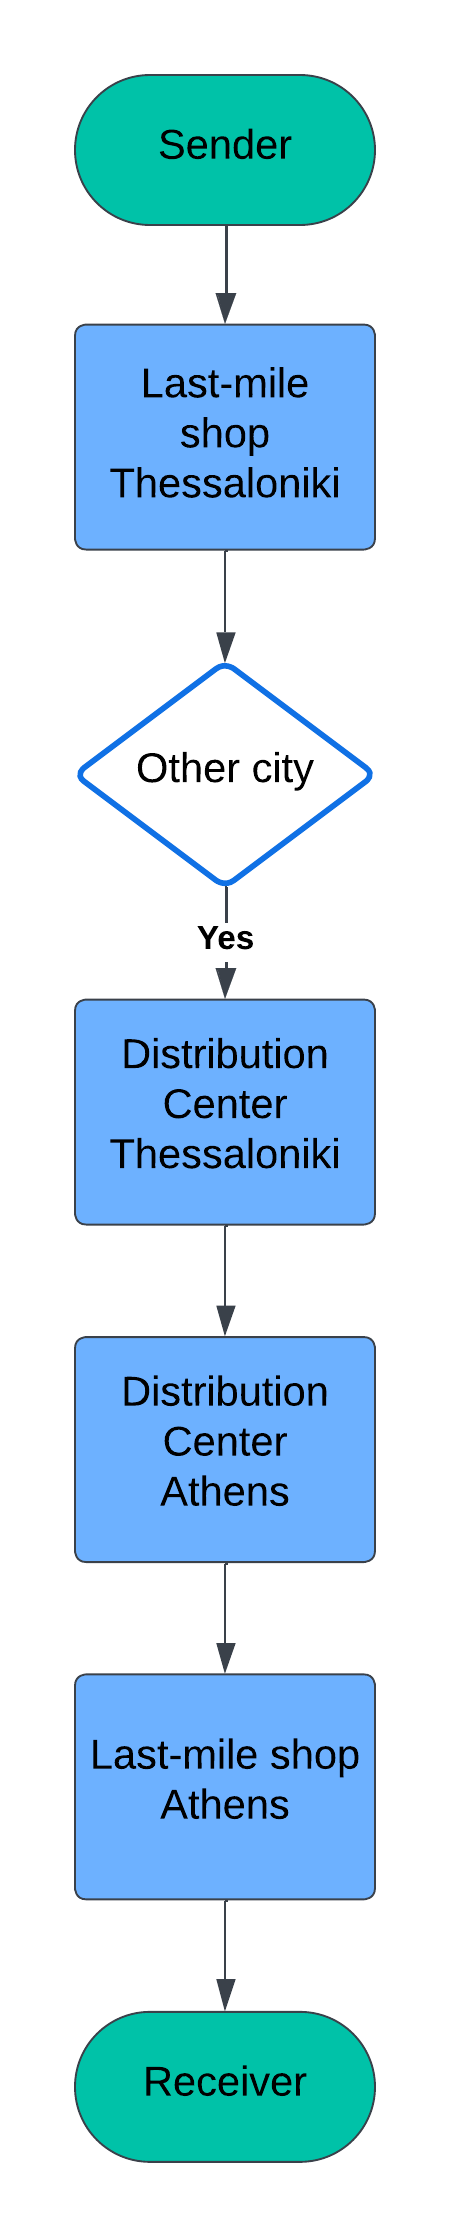
\includegraphics[width=0.5\columnwidth, height=\textheight]{Use-case-flowchart}
		\centering
	\end{figure}
	
	\section{Pseudocode for the MD-mfcmTSP}
	At the end of Algorithm 1, a local optimization function (3) is called which in addition to moving nodes in different places in the same route, also moves nodes between routes of different depots and different vehicle types.\;
	\begin{algorithm}
		\small
		\caption{MD-mfcmTSP heuristic}
		\label{alg:MDmfcmTSP}
		\KwIn{$G_T, G_M, ..., G_D$}
		\KwOut{$M_{total}$, $Sol = \{Sol^i = \{R_T^i, R_M^i, ...,R_D^i\}, Sol^{i+1}, ..., Sol^m\}$ for each $i\in D$}
		
		Create clusters $K^i$ of customer nodes for each depot $d^i\in D$\;
		by assigning each customer to the closest possible depot\;
		\For{each $d^i\in D$}{
			
			Call $Initialization(d^i, K^i)$\;
			\While{$(M_T^i > M_M^i\parallel M_T^i > M_D^i)$ $\&\&$ $stop\neq true$}{
				$diff_M = M_T^i - M_M^i$\;
				$diff_D = M_T^i - M_D^i$\;
				\uIf{$diff_M\ge diff_D$}{
					$vt = M$\;
					$cap =$ Motorbike's capacity\;
				}\Else{
					$vt = D$\;
					$cap =$ 1\;
				}
				$M_{min} = M_T^i$\;
				$r_{best} = \emptyset$\;
				\For{$j=1$ to $|R_T^i| - cap$}{
					$successive\_nodes = \emptyset$\;
					$load = 0$\;
					\While{$load + v_j^{demand} \leq cap$ $\&\&$ $v_j\in G_{vt}$}{
						$successive\_nodes \pluseq v_j$\;
					}
					\If{$|successive\_nodes| == cap$}{
						$r_{new} = R_T^i[0] + \{successive\_nodes\} + R_T^i[0]$\;
						${R'}_{vt}^i = R_{vt}^i + r_{new}$\;
						${M'}_{vt} = {R'}_{vt}^i$ 's makespan\;
						${R'}_T^i = R_T^i - \{successive\_nodes\}$\;
						${M'}_T = {R'}_T^i$ 's makespan\;
						$M_{max} = MAX({M'}_T, {M'}_{vt})$\;
						\If{$M_{max} < M_{min}$}{
							$M_{min} = M_{max}$\;
							$r_{best} = r_{new}$\;
						}
						$r_{new} = \emptyset$\;
					}
					$j\pluseq 1$\;
				}
				\uIf{$M_{min} < R_T^i$}{
					$R_T^i = R_T^i - \{r_{best}^{customers}\}$\;
					$M_T = R_T^i$ 's makespan\;
					$R_{vt}^i\pluseq r_{best}$\;
					$M_{vt} = R_{vt}^i$ 's makespan\;
					Call $local\_optimization(R_T^i, n_{max})$\;
					Call $local\_optimization(R_{vt}^i, n_{max})$\;
				}\Else{ 
					$stop = true$\;
				}
			}
			$Sol^i = \{R_T^i, R_M^i, ..., R_D^i\}$\;
		}
		$M_T = MAX(M_T^i, M_T^{i+1}, ..., M_T^m)$\;
		$M_M = MAX(M_M^i, M_M^{i+1}, ..., M_M^m)$\;
		$M_D = MAX(M_D^i, M_D^{i+1}, ..., M_D^m)$\;
		$M_{total} = MAX(M_T, M_M, ..., M_D)$\;
		Call $local\_opt\_full(Sol, n_{max})$
	\end{algorithm}

	\begin{algorithm}
		\small
		\caption{Initialization($d^i, K^i$)}
		\label{alg:initialization}
		\While{$\{K^i\}\cap \{G_T\}\neq \emptyset$}{
			$R_T^i\pluseq NearestNeighbour(\{K^i\}\cap \{G_T\})$\;
		}
		$M_T^i = R_T^i$ 's makespan\;
		$v_{free} = \{K^i\} - \{G_T\}$\;
		\uIf{$v_{free} = \emptyset$}{
			\Return{$R_T^i$}\;
		}\Else{
			\While{$v_{free}\neq \emptyset$}{
				\uIf{$M_T - M_M\geq M_T - M_D \parallel G_D = \emptyset$}{
					$R_M^i\pluseq NearestNeighbour(\{K^i\}\cap \{G_M\})$\;
					$v_{free} = v_{free} - \{R_M^i\}$\;
					$M_M^i = R_M^i$ 's makespan\;
				}\Else{
					$R_D^i\pluseq closest(\{K^i\}\cap \{G_D\})$\;
					$M_D^i = R_D^i$ 's makespan\;
				}
			}
		}
		\Return{$Sol^i$}\;
	\end{algorithm}
	
	\begin{algorithm}
		\small
		\caption{$local\_opt\_full(Sol, n_{max})$}
		Call $vt\_optimization(Sol, n_{max} = 2)$\;
		\For{each $vt$}{
			\For{each $i\in D$}{
				Call $local\_optimization(R_{vt}^i, n_{max}=2)$\;
			}
			$M_{vt} = MAX(R_{vt}^i, R_{vt}^{i+1}, ..., R_{vt}^m)$\;
			Call $mutual\_optimization(R_{vt}, n_{max}=2)$\;
		}
		Call $vt\_optimization(Sol, n_{max} = 2)$\;
	\end{algorithm}
	
	\begin{algorithm}
		\small
		\caption{$local\_optimization(r, n_{max})$}
		\For{$n=1$ to $n_{max}$}{
			\ForEach{combination of $n$ successive nodes on the route}{
				move the node(s) to a different place on the same route\;
				evaluate the new route\;
				\uIf{this route is better than the original and all constraints are satisfied}{
					replace the original route with the new one\;
				}
				continue in point 3 unless all possible places in the route have been evaluated\;
			}
		}
		\Return{$r$}\;
	\end{algorithm}
	
	\begin{algorithm}
		\small
		\caption{$mutual\_optimization(R_{vt}, n_{max})$}
		\For{$n = 1$ to $n_{max}$}{
			\ForEach{possible pair of depots $c1$ and $c2$}{
				\ForEach{combination of $n$ successive nodes in the route of c1}{
					remove the nodes from the route of c1 and insert them into c2\;
					evaluate the newly-created routes\;
					\uIf{$MAX(|{R'}_{vt}^{c1}|, |{R'}_{vt}^{c2}|) < MAX(|{R}_{vt}^{c1}|, |{R}_{vt}^{c2}|)$ and all constraints are satisfied}{
						replace the original routes with the new ones\;
					}
					continue in point 4 unless all possible places in c2 have been evaluated\;
				}
			}
		}
		\Return{$R_{VT}$}\;
	\end{algorithm}
	
	\begin{algorithm}
		\small
		\caption{$vt\_optimization(Sol, n_{max})$}
		\For{$n = 1$ to $n_{max}$}{
			\ForEach{depot $i\in D$}{
				\ForEach{possible pair of vehicle types $t1,t2\in VT$}{
					\ForEach{combination of $n$ successive nodes in $R_{t1}^i$}{
						remove the nodes from $R_{t1}^i$ and insert them in $R_{t2}^i$\;
						\uIf{$MAX(|{R'}_{t1}^i|, |{R'}_{t2}^i|) < MAX(|{R}_{t1}^i|, |{R}_{t2}^i|)$ and all constraints are satisfied}{
						replace the original routes with the new ones\;
						}
						continue in point 5 unless all possible places in $R_{t2}^i$ have been evaluated\;
					}
				}
			}
		}
		\Return{$Sol$}\;
	\end{algorithm}
	\clearpage
	% Please add the following required packages to your document preamble:
% \usepackage{booktabs}
% \usepackage{graphicx}
\begin{table*}[!ht]
	\centering
	\caption{Local optimization impact on heuristic using proximity clustering}
	\resizebox{\textwidth}{!}{%
		\begin{tabular}{@{}cccccccccc@{}}
			\toprule
			\textbf{Instance} & \textbf{Best} & \textbf{Full Local Opt} & \textbf{gap(\%)} & \textbf{No Local Opt} & \textbf{gap(\%)} & \textbf{Final Only} & \textbf{gap(\%)} & \textbf{Swap Only} & \textbf{gap(\%)} \\ 
			\midrule
			p01-C & 215.15 & 217.42 & 1.06 & 334.04 & 55.26 & \textbf{215.15} & 0.00 & 173.96 & 27.33 \\ \midrule
			p02-C & 218.4 & 219.20 & 0.37 & 308.83 & 41.41 & \textbf{218.40} & 0.00 & 289.58 & 32.59 \\ \midrule
			p03-C & 202.43 & 214.84 & 6.13 & 253.18 & 25.07 & \textbf{202.43} & 0.00 & 255.52 & 26.23 \\ \midrule
			p04-C & 668.81 & \textbf{668.81} & 0.00 & 779.34 & 16.53 & 711.80 & 6.43 & 691.62 & 3.41 \\ \midrule
			p05-C & 630.78 & \textbf{630.78} & 0.00 & 726.62 & 15.19 & 655.4 & 3.90 & 697.86 & 10.63 \\ \midrule
			p06-C & 431.32 & 435.42 & 0.95 & 650.32 & 50.77 & \textbf{431.32} & 0.00 & 564.79 & 30.94 \\ \midrule
			p07-C & 309.48 & \textbf{309.48} & 0.00 & 350.77 & 13.34 & 349.19 & 12.83 & 366.51 & 18.43 \\ \midrule
			p08-C & 3079.58 & 3333.93 & 8.26 & 3321.63 & 7.86 & \textbf{3079.58} & 0.00 & 3428.15 & 11.32 \\ \midrule
			p09-C & 1917.82 & \textbf{1917.82} & 0.00 & 2429.24 & 26.67 & 2102.98 & 9.65 & 2303.70 & 20.12 \\ \midrule
			p10-C & 1493.13 & \textbf{1493.13} & 0.00 & 1864.23 & 24.85 & 1525.37 & 2.16 & 1706.14 & 14.27 \\ \midrule
			p11-C & 1101.33 & 1145.75 & 4.03 & 1239.36 & 12.53 & \textbf{1101.33} & 0.00 & 1276.59 & 15.91 \\ \midrule
			p12-C & 1273.77 & \textbf{1273.77} & 0.00 & 1356.09 & 6.46 & 1307.11 & 2.62 & \textbf{1273.77} & 0.00 \\ \midrule
			p13-C & 1191.96 & 1226.63 & 2.91 & 1455.87 & 22.14 & \textbf{1191.96} & 0.00 & 1259.97 & 5.71 \\ \midrule
			p14-C & 1248.53 & 1284.73 & 2.90 & 1413.87 & 13.24 & \textbf{1248.53} & 0.00 & 1302.34 & 4.31 \\ \midrule
			p15-C & 1347.67 & \textbf{1347.67} & 0.00 & 1508.50 & 11.93 & 1355.08 & 0.55 & 1375.95 & 2.10 \\ \midrule
			p16-C & 1289.29 & \textbf{1289.29} & 0.00 & 1448.53 & 12.35 & 1328.00 & 3.00 & \textbf{1289.29} & 0.00 \\ \midrule
			p17-C & 1282.38 & 1320.91 & 3.00 & 1375.55 & 7.27 & \textbf{1282.38} & 0.00 & 1320.91 & 3.00 \\ \midrule
			p18-C & 1260.24 & \textbf{1260.24} & 0.00 & 1446.92 & 14.81 & 1317.54 & 4.55 & 1339.83 & 6.32 \\ \midrule
			p19-C & 1266.92 & \textbf{1266.92} & 0.00 & 1406.13 & 10.99 & 1289.95 & 1.82 & 1301.62 & 2.74 \\ \midrule
			p20-C & 1323.1 & \textbf{1323.10} & 0.00 & 1429.00 & 8.00 & 1338.42 & 1.16 & 1351.39 & 2.14 \\ \midrule
			p21-C & 1309.14 & 1363.18 & 4.13 & 1470.03 & 12.29 & \textbf{1309.14} & 0.00 & 1363.18 & 4.13 \\ \midrule
			p22-C & 1295.67 & \textbf{1295.67} & 0.00 & 1465.74 & 13.13 & 1351.96 & 4.34 & 1306.6 & 0.84 \\ \midrule
			p23-C & 1252.36 & \textbf{1252.36} & 0.00 & 1396.11 & 11.48 & 1262.65 & 0.82 & 1254.42 & 0.16 \\ \midrule
			\textbf{AVG} & 1113.44 & \textbf{1134.39} & \textbf{1.46} & 1279.56 & 18.85 & 1138.07 & 2.34 & 1199.72 & 10.54 \\ \bottomrule
		\end{tabular}%
	}
\end{table*}\;
	% Please add the following required packages to your document preamble:
% \usepackage{booktabs}
% \usepackage{graphicx}
\begin{table*}[!ht]
	\begin{minipage}{\columnwidth}
		\centering
		\caption{AACONC+ Results}
	\resizebox{\textwidth}{!}{%
		\begin{tabular}{@{}ccccccc@{}}
			\toprule
			\textbf{Instance} & \textbf{Best} & \textbf{Average} & \textbf{gap(\%)} & \textbf{Worst} & \textbf{gap(\%)} & \textbf{Average time(s)} \\
			\midrule
			p01-C & 178.56 & 196.74 & 10.18 & 225.60 & 26.34 & 141 \\
			\midrule
			p02-C & 172.73 & 196.57 & 13.8 & 234.78 & 35.92 & 123 \\
			\midrule
			p03-C & 173.82 & 187.26 & 7.73 & 210.15 & 20.90 & 305 \\
			\midrule
			p04-C & 629.88 & 644.84 & 2.37 & 675.63 & 7.26 & 1203 \\
			\midrule
			p05-C & 573.03 & 613.47 & 7.06 & 692.44 & 20.84 & 884 \\
			\midrule
			p06-C & 379.10 & 390.34 & 2.96 & 403.39 & 6.41 & 1316 \\
			\midrule
			p07-C & 288.24 & 297.91 & 3.35 & 314.78 & 9.21 & 798 \\
			\midrule
			p08-C & 3023.77 & 3100.23 & 2.53 & 3265.97 & 8.01 & 1635 \\
			\midrule
			p09-C & 1705.03 & 1774.86 & 4.10 & 1846.92 & 8.32 & 3391 \\
			\midrule
			p10-C & 1286.28 & 1319.78 & 2.60 & 1349.47 & 4.91 & 3549 \\
			\midrule
			p11-C & 992.16 & 1035.63 & 4.38 & 1061.7 & 7.01 & 3600 \\
			\midrule
			p12-C & 1082.12 & 1123.30 & 3.81 & 1175.39 & 8.62 & 446 \\
			\midrule
			p13-C & 1099.02 & 1135.30 & 3.30 & 1191.96 & 8.46 & 491 \\
			\midrule
			p14-C & 1111.12 & 1123.33 & 1.10 & 1170.17 & 5.31 & 423 \\
			\midrule
			p15-C & 1166.08 & 1202.57 & 3.13 & 1228.27 & 5.33 & 2471 \\
			\midrule
			p16-C & 1178.51 & 1209.60 & 2.64 & 1241.67 & 5.36 & 2146 \\
			\midrule
			p17-C & 1142.74 & 1199.88 & 5.00 & 1253.47 & 9.69 & 2628 \\
			\midrule
			p18-C & 1231.96 & 1263.90 & 2.59 & 1296.42 & 5.23 & 3368 \\
			\midrule
			p19-C & 1250.26 & 1266.54 & 1.30 & 1284.23 & 2.72 & 3600 \\
			\midrule
			p20-C & 1246.36 & 1266.70 & 1.63 & 1280.77 & 2.76 & 3445 \\
			\midrule
			p21-C & 1296.19 & 1330.11 & 2.62 & 1347.09 & 3.93 & 3600 \\
			\midrule
			p22-C & 1317.94 & 1332.07 & 1.07 & 1354.61 & 2.78 & 3600 \\
			\midrule
			p23-C & 1319.93 & 1341.50 & 1.63 & 1356.62 & 2.78 & 3600 \\
			\midrule
			\textbf{Average} & 1037.52 & 1067.59 & 3.46 & 1107.25 & 8.68 & 2021.13 \\ \bottomrule
		\end{tabular}%
	}
	\label{tab:table2}
\end{minipage}
\end{table*}\;
	% Please add the following required packages to your document preamble:
% \usepackage{booktabs}
% \usepackage{graphicx}
\begin{table*}[!ht]
		\centering
	\caption{Local optimization impact on heuristic using k-means clustering}
	\resizebox{\textwidth}{!}{%
		\begin{tabular}{@{}cccccccccc@{}}
			\toprule
			\textbf{Instance} & \textbf{Best} & \textbf{Full Local Opt} & \textbf{gap(\%)} & \textbf{No Local Opt} & \textbf{gap(\%)} & \textbf{Final Only} & \textbf{gap(\%)} & \textbf{Swap Only} & \textbf{gap(\%)} \\ \midrule
			p01 & \textbf{191.03} & \textbf{191.03} & 0.00 & 225.72 & 18.16 & 202.96 & 6.25 & 201.60 & 5.53 \\
			\midrule
			p02 & \textbf{187.17} & 188.60 & 0.76 & 209.39 & 11.87 & \textbf{187.17} & 0.00 & 198.02 & 5.80 \\
			\midrule
			p03 & \textbf{185.82} & \textbf{185.82} & 0.00 & 200.64 & 7.98 & 188.63 & 1.51 & 198.01 & 6.56 \\
			\midrule
			p04 & \textbf{694.96} & \textbf{694.96} & 0.00 & 807.71 & 16.22 & 700.95 & 0.86 & \textbf{694.96} & 0.00 \\
			\midrule
			p05 & \textbf{624.33} & \textbf{624.33} & 0.00 & 695.79 & 11.45 & 629.61 & 0.85 & 642.77 & 2.95 \\
			\midrule
			p06 & \textbf{416.25} & \textbf{416.25} & 0.00 & 492.31 & 18.27 & 417.09 & 0.20 & 456.81 & 9.74 \\
			\midrule
			p07 & \textbf{313.57} & 314.41 & 0.27 & 359.30 & 14.58 & \textbf{313.57} & 0.00 & 339.09 & 8.14 \\
			\midrule
			p08 & \textbf{3051.63} & 3186.02 & 4.40 & 3288.45 & 7.76 & \textbf{3051.63} & 0.00 & 3256.46 & 6.71 \\
			\midrule
			p09 & \textbf{1932.21} & 1964.49 & 1.67 & 2099.99 & 8.68 & \textbf{1932.21} & 0.00 & 2031.19 & 5.12 \\
			\midrule
			p10 & \textbf{1463.63} & 1500.38 & 2.51 & 1636.23 & 11.79 & \textbf{1463.63} & 0.00 & 1658.74 & 13.33 \\
			\midrule
			p11 & \textbf{1031.09} & \textbf{1031.09} & 0.00 & 1209.73 & 17.33 & 1060.37 & 2.84 & 1080.39 & 4.78 \\
			\midrule
			p12 & \textbf{1273.77} & \textbf{1273.77} & 0.00 & 1356.09 & 6.46 & 1307.11 & 2.62 & \textbf{1273.77} & 0.00 \\
			\midrule
			p13 & \textbf{1191.96} & 1226.63 & 2.91 & 1455.87 & 22.14 & \textbf{1191.96} & 0.00 & 1259.97 & 5.71 \\
			\midrule
			p14 & \textbf{1248.53} & 1284.73 & 2.90 & 1413.87 & 13.24 & \textbf{1248.53} & 0.00 & 1302.34 & 4.31 \\
			\midrule
			p15 & \textbf{1295.23} & \textbf{1295.23} & 0.00 & 1434.72 & 10.77 & 1303.76 & 0.66 & \textbf{1295.23} & 0.00 \\
			\midrule
			p16 & \textbf{1289.29} & \textbf{1289.29} & 0.00 & 1436.36 & 11.41 & 1328.00 & 3.00 & \textbf{1289.29} & 0.00 \\
			\midrule
			p17 & \textbf{1273.39} & \textbf{1273.39} & 0.00 & 1375.55 & 8.02 & 1282.38 & 0.71 & 1283.38 & 0.78 \\
			\midrule
			p18 & \textbf{1211.56} & \textbf{1211.56} & 0.00 & 1369.81 & 13.06 & 1243.53 & 2.64 & 1280.85 & 5.72 \\
			\midrule
			p19 & \textbf{1248.93} & \textbf{1248.93} & 0.00 & 1384.13 & 10.83 & 1263.35 & 1.15 & 1281.68 & 2.62 \\
			\midrule
			p20 & \textbf{1234.12} & \textbf{1234.12} & 0.00 & 1389.60 & 12.60 & 1256.25 & 1.79 & 1267.53 & 2.71 \\
			\midrule
			p21 & \textbf{1231.23} & \textbf{1231.23} & 0.00 & 1354.91 & 10.05 & 1261.89 & 2.49 & 1278.10 & 3.81 \\
			\midrule
			p22 & \textbf{1230.99} & \textbf{1230.99} & 0.00 & 1379.49 & 12.06 & 1250.49 & 1.58 & 1265.17 & 2.78 \\
			\midrule
			p23 & \textbf{1222.63} & \textbf{1222.63} & 0.00 & 1363.52 & 11.52 & 1233.67 & 0.90 & 1250.29 & 2.26 \\
			\midrule
			Average & \textbf{1088.84} & 1100.86 & 0.67 & 1214.75 & 12.45 & 1100.81 & 1.31 & 1134.16 & 4.32 \\
			\bottomrule
		\end{tabular}%
	}

\end{table*}
\;
	\onecolumn
	\captionsetup{justification=centering}  % Center the captions
	\begin{figure}[t]
		\centering
		\caption{Comparison to the best solution found by AACONC+}
		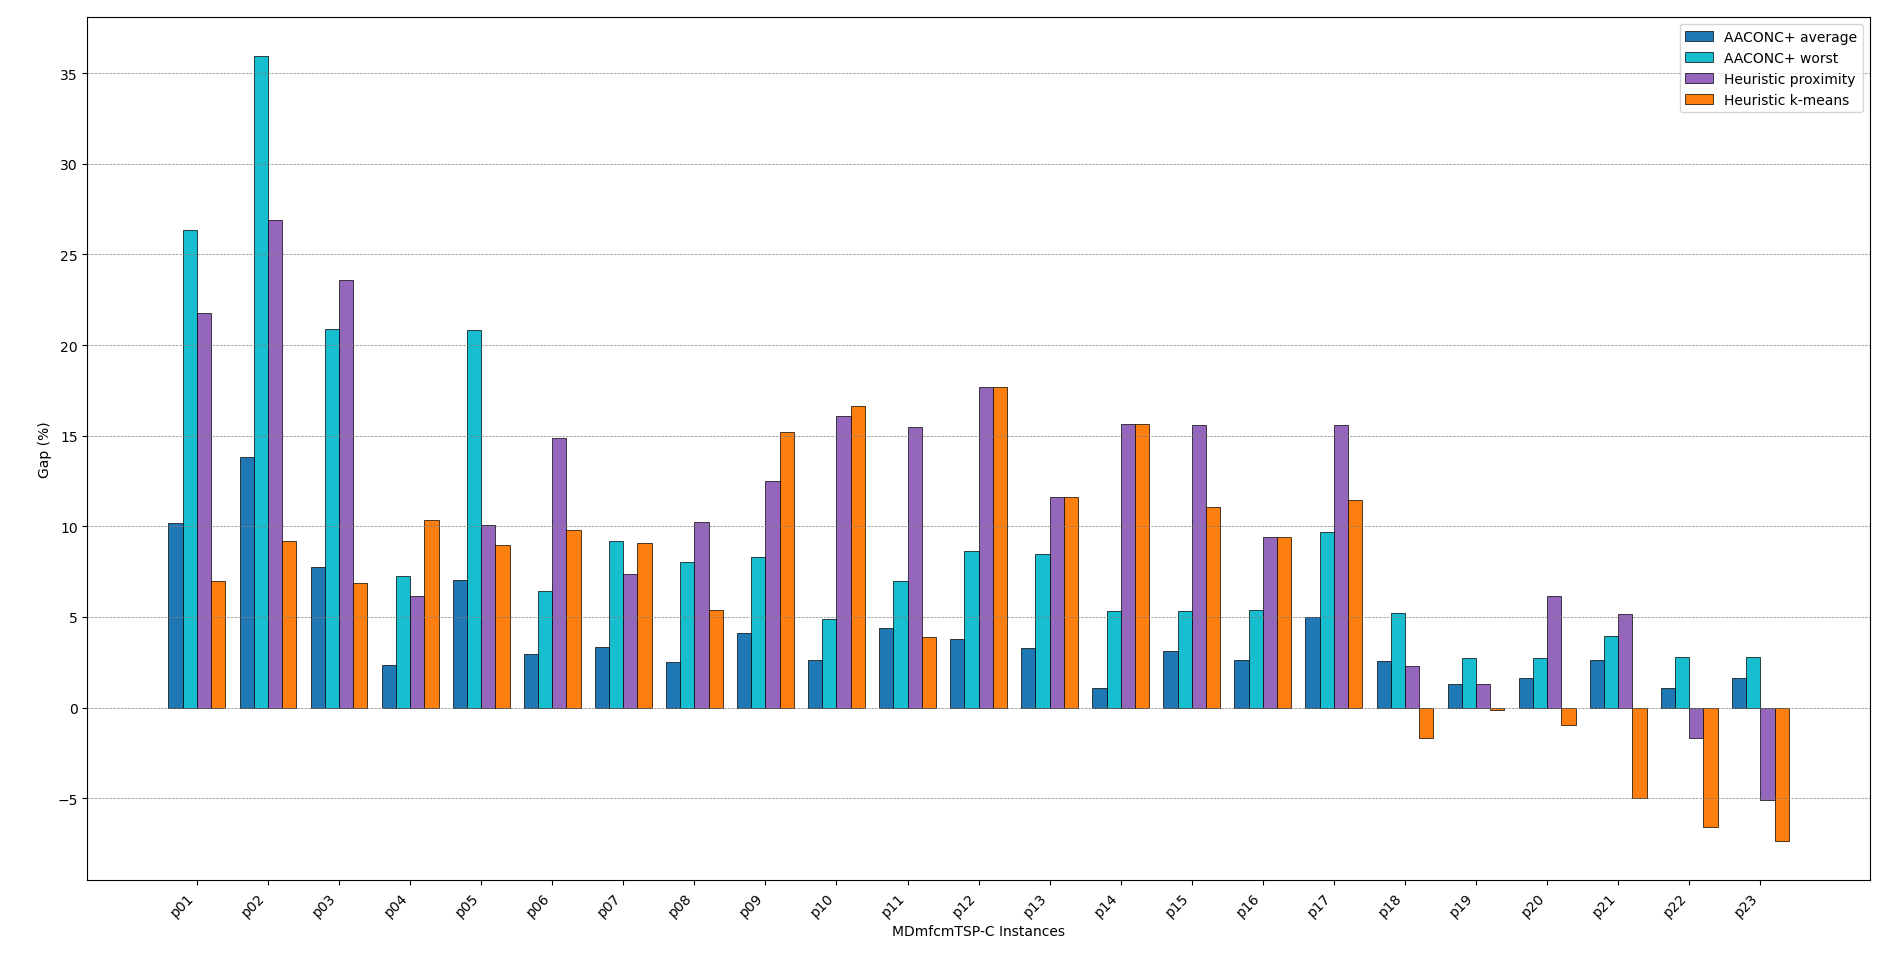
\includegraphics[width=\textwidth]{gaps_to_aco_best}
	\end{figure}
	\begin{figure}[t]
		\caption{Comparison to full local optimization (proximity clustering)}
		\centering
		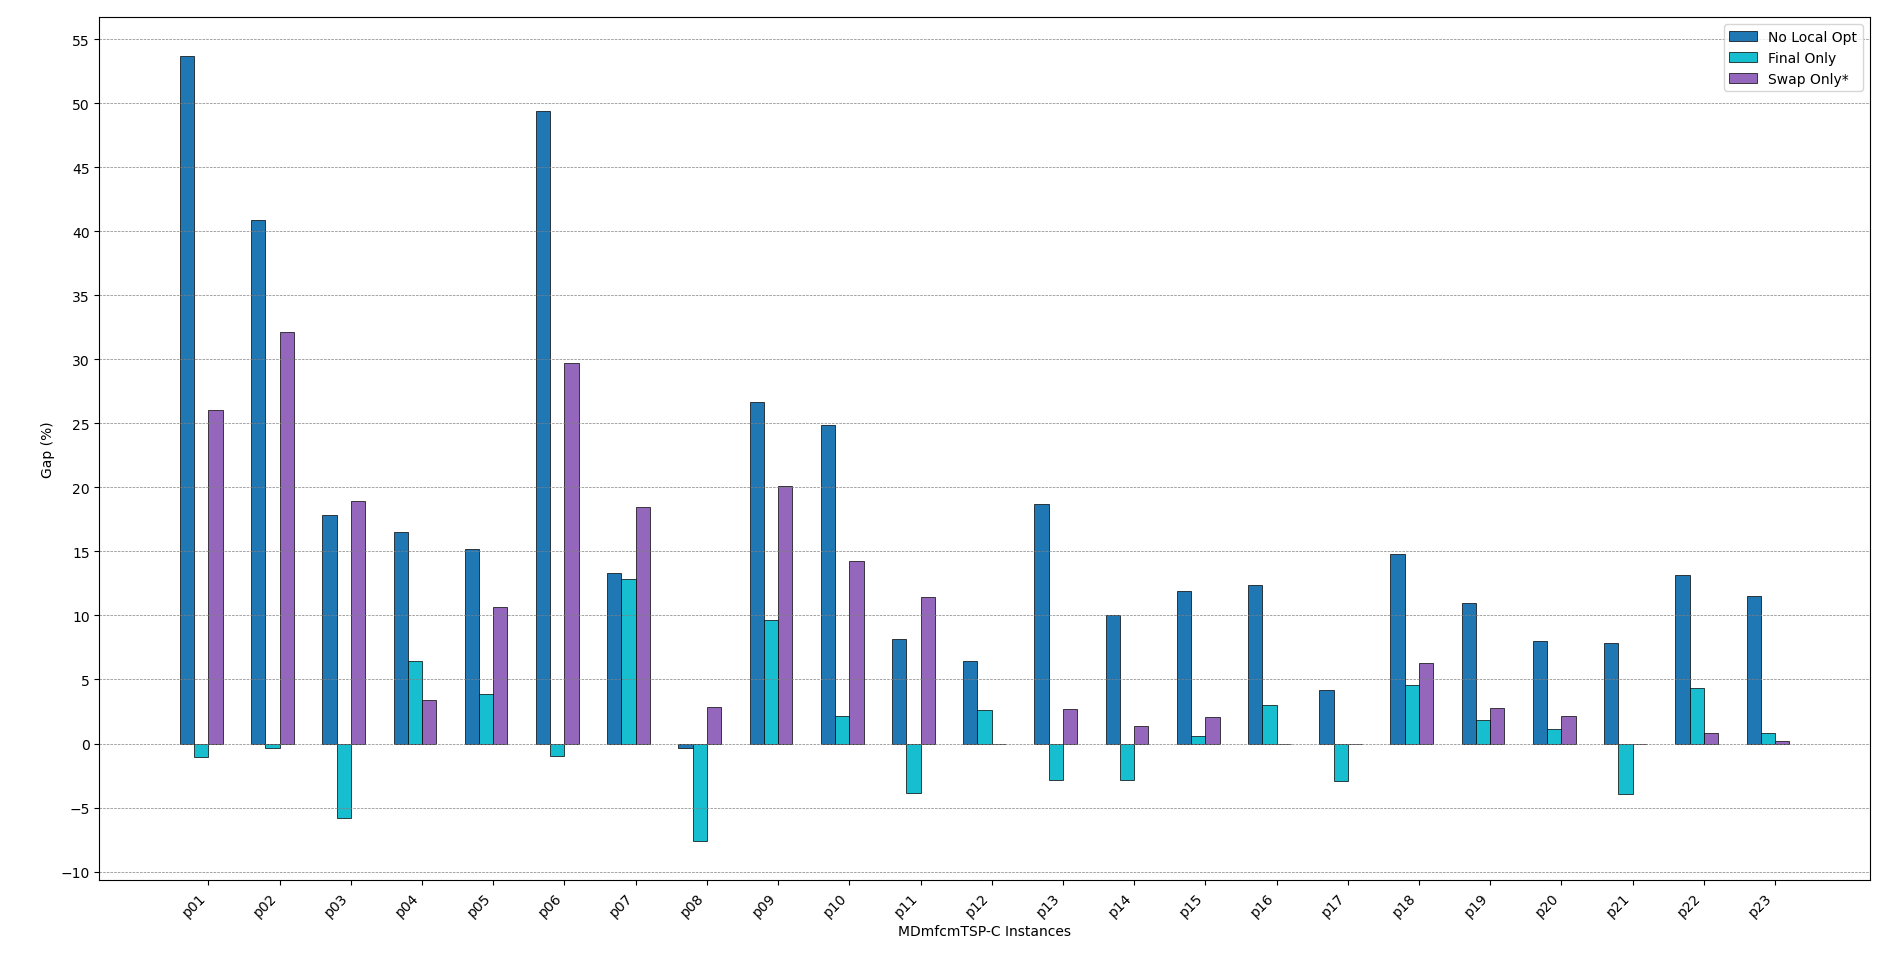
\includegraphics[width=\textwidth]{local_opt_comp_to_full}
	\end{figure}
	\begin{figure}[t]
		\caption{Comparison to full local optimization (k-means clustering)}
		\centering
		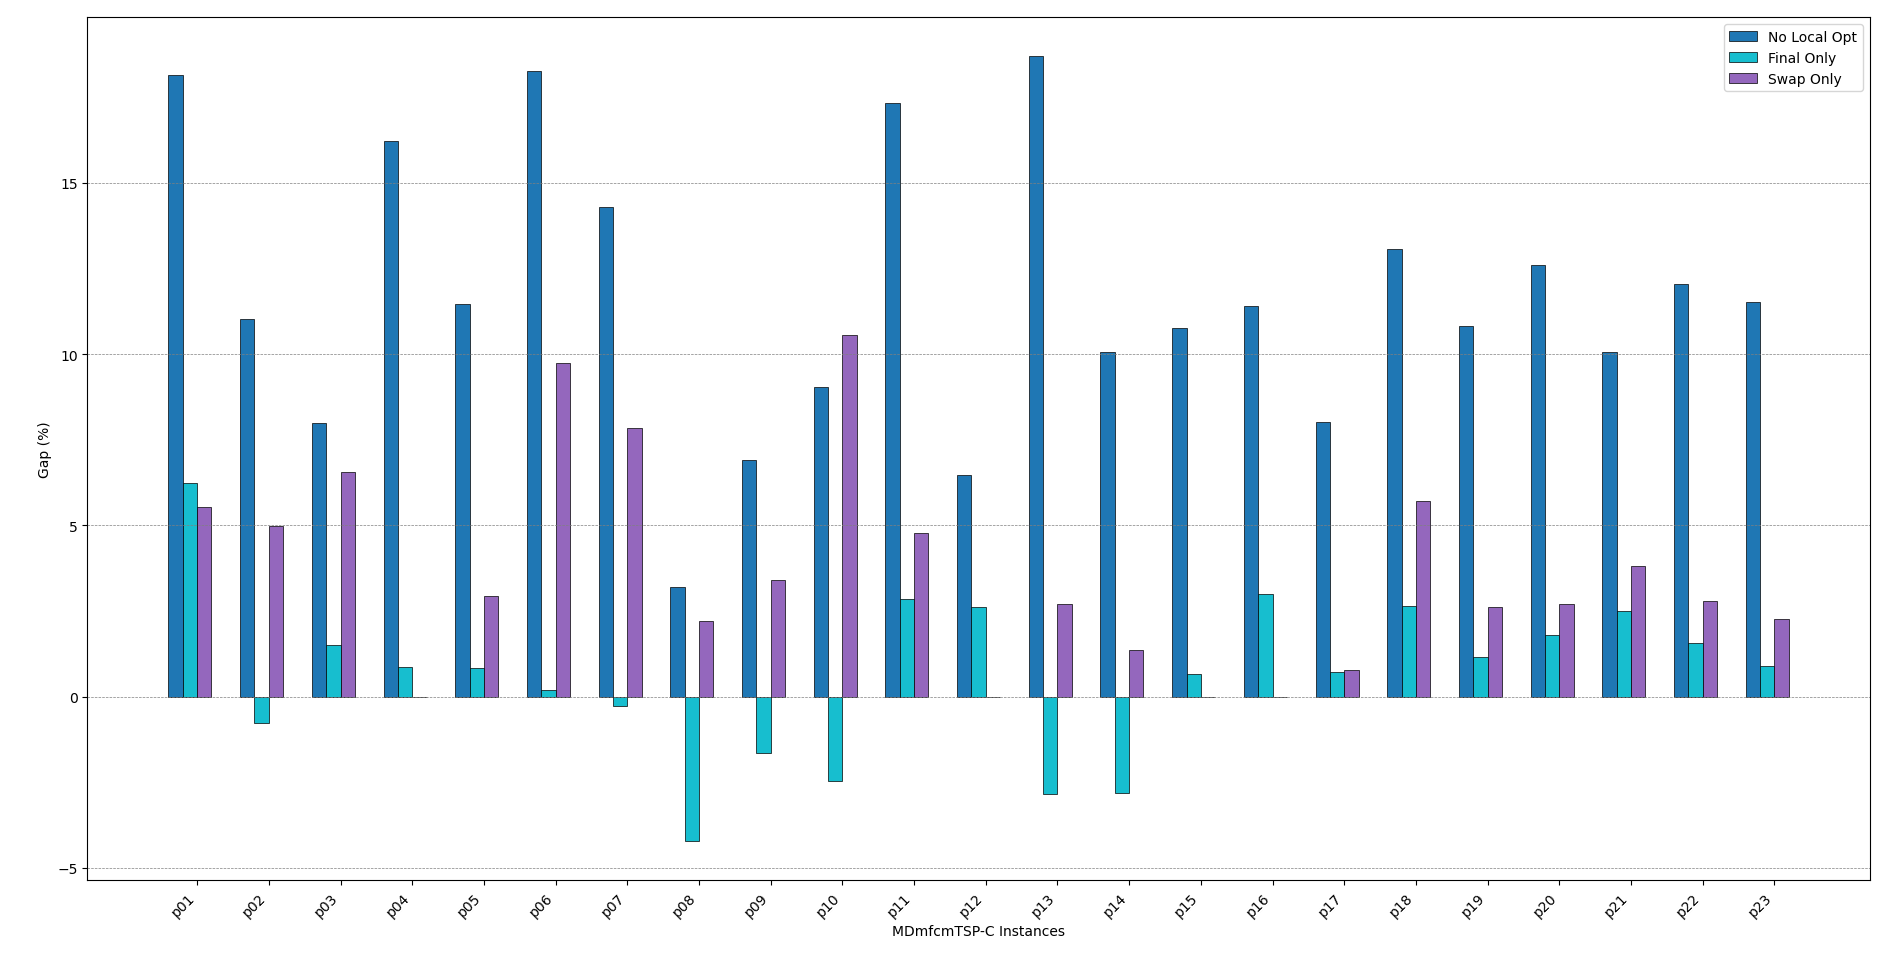
\includegraphics[width=\textwidth]{local_opt_comp_to_full_kmeans}
	\end{figure}
	\begin{figure}[t]
		\caption[width=\textwidth]{kmeans Clustering}
		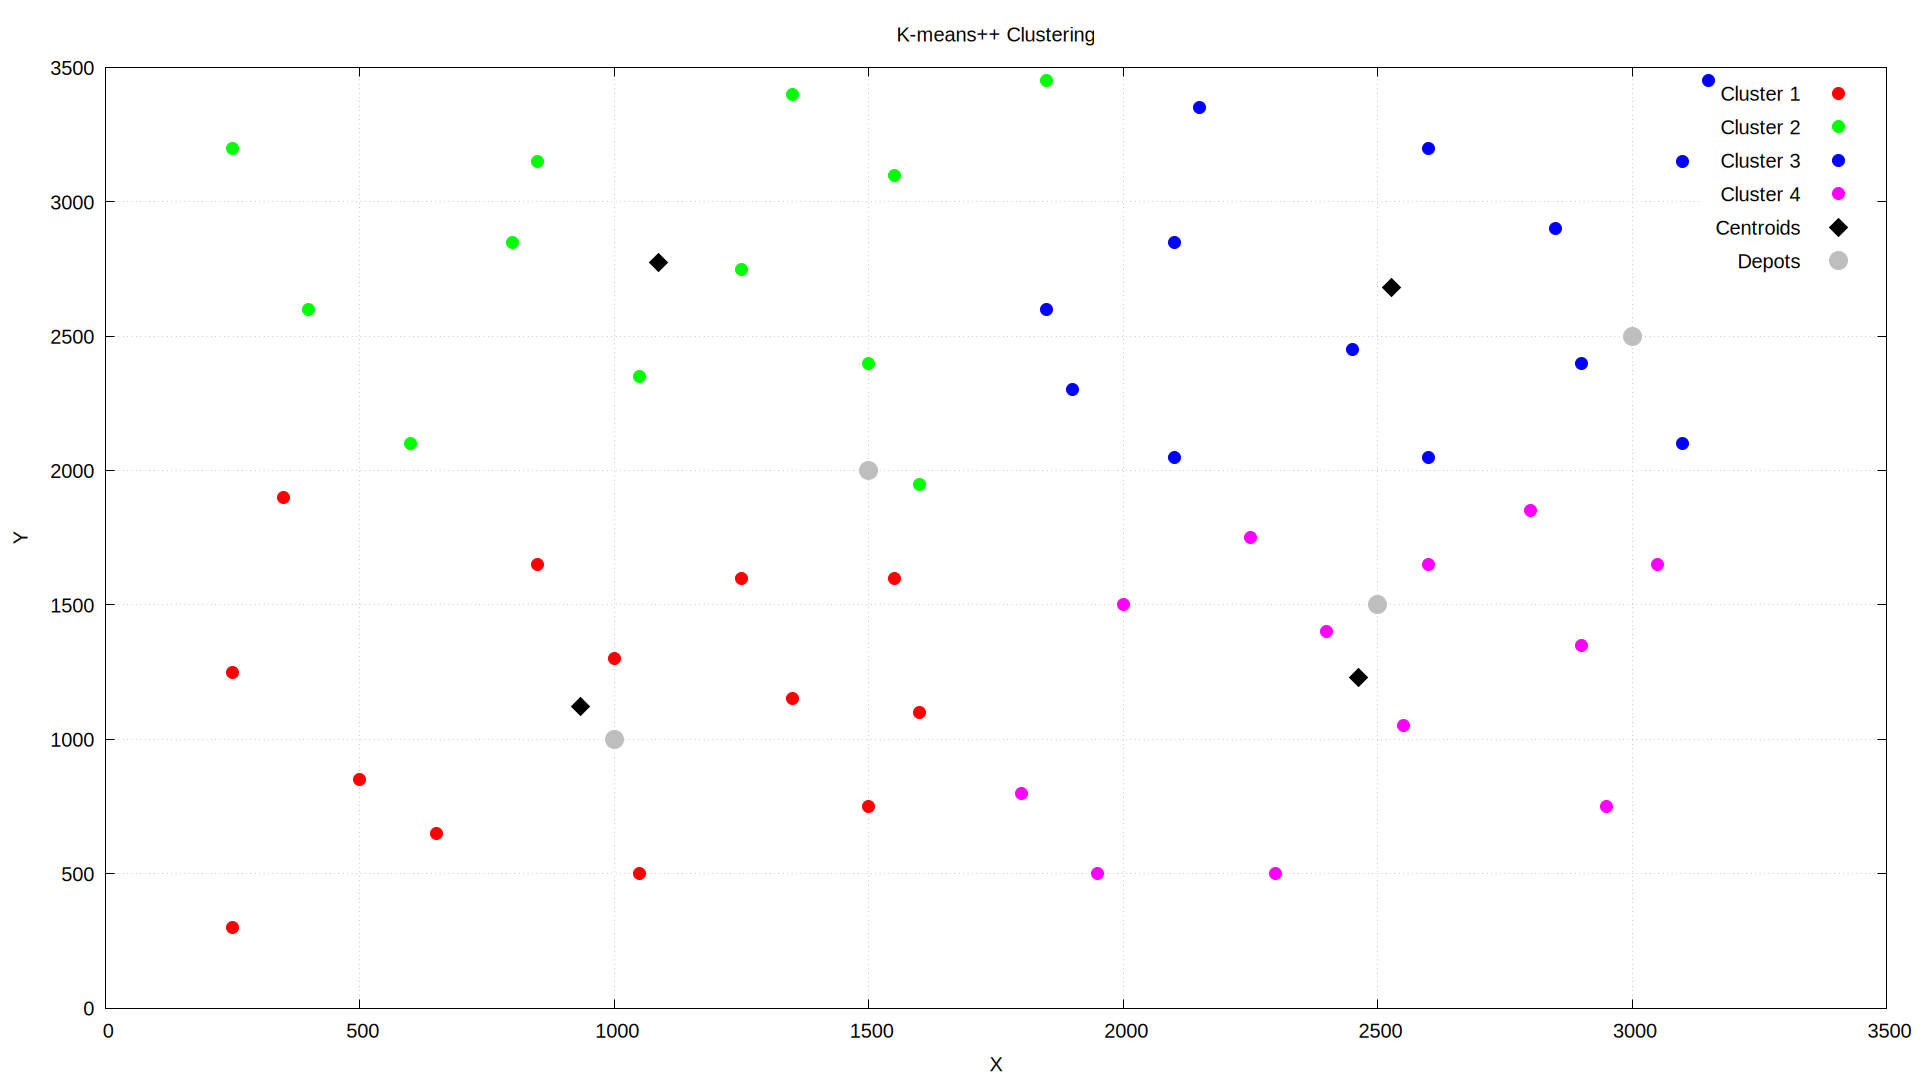
\includegraphics[width=\textwidth]{kmeans-01}
		\centering
	\end{figure}
	\twocolumn
	\section{Experiment results}
	\subsection{Algorithms comparison}
	The objective value (measure in seconds), which is the total tour time of the delivery service, and four other performance indicators are detailed reported in Appendix 1. For each heuristic approach, such as GA, SA, or OR-Tools, we summarize the average values of the total tour time of 30 iterations for each setting, i.e., urban, suburban, and countryside areas. The results indicate that OR-Tools achieves the best outcomes among algorithms in our experiment. The mean difference of each instance upon three heuristic approaches is further checked by ANOVA-F testing, 87\% of cases then show the mean differences are
	significant at least $\alpha$ = 5 \% (OR-Tools values in bold). The results are presented in Appendix 2. We note that TSP-0D denotes the truck only and TSP-1D to TSP-5D stands for one to five drones equipped with the truck. We then analyze the outcomes in the rest of the article following the OR-Tools.
	
	
	\section{Conclusion}
	This novel routing problem contributes to logistics research by offering a new perspective on urban delivery systems. Unlike traditional models with fixed capacities and single vehicle types, this problem accounts for multiple vehicle types and depots with unlimited parcel supplies. 
	\par 
	The insights gained from solving this problem can enhance operational efficiency in real-world scenarios, such as:
	\begin{itemize}
		\item Optimized Vehicle Utilization: Efficiently managing different types of vehicles to reduce delivery times and operational costs.
		\item Scalable Solutions: Developing algorithms that can handle large-scale urban delivery networks with multiple depots and dynamic customer demands.
		\item Sustainable Logistics: Promoting the use of environmentally friendly vehicles like drones and motorbikes for last-mile delivery, reducing carbon footprints.
	\end{itemize}
	By addressing these aspects, the research offers practical solutions for improving parcel delivery systems, making it highly relevant for logistics companies seeking to enhance their service efficiency in densely populated urban areas.
	

\end{document}